%  \documentclass[DIV=12, a4]{scrartcl}
%\documentclass[12pt, a5]{scrartcl}

% \documentclass[a4paper]{report}
% \usepackage[
% % fancytheorems, 
% noindent, 
% %spacingfix, 
% %noheader
% ]{vanilla}


\documentclass[a4paper]{scrartcl}
\usepackage[
fancytheorems, 
noindent, 
% %spacingfix, 
% %noheader,
fancyproofs
]{adam} 

\usepackage{tikz}
\usepackage{booktabs}

% \usepackage{subfig}


\title{Groups, Rings and Modules}
% \subtitle{Adam Kelly}
\author{Adam Kelly}
% \date{Michaelmas 2020}
\date{\today}

\begin{document}

\maketitle

% \newcommand{\newchapter}{\chapter}
% \newcommand{\newsection}{\section}
% \newcommand{\newsubsection}{\subsection}
% \newcommand{\newsubsubsection}{\subsubsection}
\newcommand{\newchapter}{\section}
\newcommand{\newsection}{\subsection}
\newcommand{\newsubsection}{\subsubsection}
\newcommand{\newsubsubsection}{\subsubsubsection}

\begin{abstract}
	
	% \vspace{2\baselineskip}
	% {\color{red} None of the notes here have been reviewed at all, and are just exactly what was taken down live in the lectures. I would turn around now and come back in a few days, when I have gone back, cleaned things up, fixed explanations and added some structure.}
	% \vspace{5\baselineskip}

	This set of notes is a work-in-progress account of the course `Groups, Rings and Modules', originally lectured by Dr Tom Fisher in Lent 2020 at Cambridge. These notes are not a transcription of the lectures, but they do roughly follow what was lectured (in content and in structure).

	These notes are my own view of what was taught, and should be somewhat of a superset of what was actually taught. I frequently provide different explanations, proofs, examples, and so on in areas where I feel they are helpful. Because of this, this work is likely to contain errors, which you may assume are my own. If you spot any or have any other feedback, I can be contacted at \href{mailto:ak2316@cam.ac.uk}{ak2316@cam.ac.uk}.


	% {\color{red} Notes written upto lecture 6.}
	% During the creation of this document, I consulted a number of other books and resources. All of these are listed in the bibliography. 

\end{abstract}

\tableofcontents

% \clearpage
% \newchapter{Introduction}



% \newsection{Structure of the Course}

% This course is, quite naturally, divided into three sections.

% \begin{enumerate}
% 	\item \emph{Groups}
	
% 	We will be continuing on from IA Groups, paying particular attention to certain topics such as simple groups, $p$-groups and $p$-subgroups. The main highlight of this part of the course will be the Sylow theorems.

% 	\item \emph{Rings}
	
% 	Rings are sets where we can add, subtract and multiply (but not necessarily divide), for example, $\Z$. A ring where division is always possible is a field, for example $\Q$, $\R$ and $\Z/p\Z$ for a prime $p$.

% 	\item \emph{Modules}
	
% 	A module is the analog of a vector space where we work over a ring, rather than a field. We will attempt to classify modules over certain `nice' rings. This will allow us to prove the Jordan Normal theorem of matrices and to classify finite abelian groups. 
% \end{enumerate}

% \newsection{Books}

% As with most mathematics courses in Cambridge, you will not need a textbook to follow this course. What is covered in lectures is enough to do both the example sheets and the examinations for this course. Still, you might find that a textbook can provide a different perspective, additional worked examples, and additional material that you may find informative, helpful or fun.

% In particular, the following books are quite relevant/good, but there is no expectation that you will look at these.

% \begin{itemize}
% 	\item P. M. Cohn, \emph{Classical Algebra}.
	
% 	This covers the whole course (but does have some weird notation).

% 	\item Hartley \& Hawkes, \emph{Rings, Modules \& Linear Algebra}.
	
% 	This is a good reference for the `rings and modules' part of the course, but notably doesn't include any content on group theory.
% \end{itemize}

% You should be able to find all of these books in either your college library or the university library.


% \clearpage


\newchapter{Groups}

The first algebraic object that we shall consider in this course is one you are likely familiar with -- a group. 

\newsection{Definitions}

We will begin by defining what a group is.

\begin{definition}[Group]
	A \vocab{group} is a pair ($G$, $*$) consisting of a set $G$ and a binary operation\footnote{Some texts include an additional \emph{closure} axiom, but this is implied by $*$ being a binary operation on $G$.} $* : G \times G \rightarrow G$ satisfying the axioms:
	\begin{itemize}
		\item \emph{Identity}. There is an element $e \in G$ such that $e * g = g * e = g$ for all $g \in G$,
		\item \emph{Inverses}. For every element $g \in G$, there is an element $g^{-1} \in G$ such that $g * g^{-1} = g^{-1} * g = e$.
		\item \emph{Associativity}. The operation $*$ is associative.
	\end{itemize}
\end{definition}

\begin{remark}
	We will usually either use additive or multiplicative notation for groups, and in these cases we will often write $0$ or $1$ for the identity respectively.
\end{remark}

\begin{definition}[Subgroup]
	A subset $H \subseteq G$ is a \vocab{subgroup} of $G$, written $H \leq G$, if it is a group with respect to the operation $*$ defined on $H \times H$.
\end{definition}

There is a way to test the conditions needed for a subset to be a subgroup in just a few lines, but it does have limited utility.

\begin{lemma}[Fast Subgroup Checking Lemma]
A nonempty subset $H \subseteq G$ is a subgroup if $a, b \in H$ implies $a * b^{-1} \in H$.
\end{lemma}
\begin{proof}[Proof Sketch]
	Check that this implies the definition.
\end{proof}

\begin{example}[Examples of Groups]
	The following are all examples of groups.
	\begin{enumerate}[label=(\roman*)]
		\item The additive groups $(\Z, +) \leq (\Q, +) \leq (\R, +)$.
		\item The cyclic group of order $n$, $C_n$.
		\item The dihedral group $D_{2n}$ of the symmetries of a regular $n$-gon.
		\item The symmetric group $S_n$ and alternating group $A_n$, where $S_n$ is the group of permutations of $\{1, 2, \dots, n\}$ and $A_n \leq S_m$ is the group of even permuations. 
		\item The quaternion group $Q_8 = \{\pm 1, \pm i, \pm j, \pm k \}$ with $i^2 = j^2 = k^2 = ijk = -1$.
		\item The matrix groups over some field $F$, $\GL_n(F)$ of all $n \times n$ matrices over $F$ with non-zero determinant, and $\SL_n(F) \leq \GL_n(F)$, the subgroup of matrices with determinant 1.
	\end{enumerate}
\end{example}

\begin{definition}[Direct Product]
	The \vocab{direct product} of groups $G$ and $H$ is $G \times H$ with operation $(g_1, h_1) * (g_2, h_2) = (g_1 g_2, h_1 h_2)$. 
\end{definition}

For a subgroup $H \leq G$, the \vocab{left cosets} of $H$ in $G$ are the sets $gH = \{gh \mid h \in H \}$ where $g \in G$. Recall that these partition $G$, and each has the same cardinality as $H$. From this we deduce Lagrange's theorem.

\begin{theorem}[Lagrange's Theorem]
	Let $G$ be a finite group, and $H$ be a subgroup. Then $|G| = |H| \cdot |G : H|$ where $|G : H|$ is the \vocab{index} of $H$ in $G$, the number of left cosets of $H$ in $G$.
\end{theorem}

It is natural to wonder whether there is a converse to Lagrange's theorem, and it turns out that the converse is \emph{not} true in general. There is a partial converse however.

\begin{theorem}[First Sylow Theorem]
	If $G$ is a group with $|G| = p^a m$ where $p$ is a prime and $p \nmid m$, then there exists $H \leq G$ with $|H| = p^a$.
\end{theorem}

We will prove this theorem later on.

\begin{definition}[Order of an Element]
	Let $G$ be a group and $g \in G$. If there exists $n \geq 1$ such that $g^n = 1$, then the least such $n$ is the \vocab{order} of $g$. If no such $n$ exists, we say $g$ hsa infinite order.
\end{definition}

\begin{remark} 
If $g$ has order $d$, then $g^n = 1 \iff d \mid n$. The proof follows from the division algorithm. Also, $\{1, g, g^2, \dots, g^{d - 1}\} \leq G$ and so if $G$ is finite, then by Lagrange, $d \mid |G|$.
\end{remark}

\begin{definition}[Normal Subgroup]
	A subgroup $H \leq G$ is \vocab{normal} if $g^{-1} H g = H$ for all $g \in G$. We write $H \normal G$ in this case.
\end{definition}

\begin{proposition}[Quotient Group]
	If $H \normal G$, then the set $G/H$ of left cosets of $H$ in $G$ is a group called the \vocab{quotient group} with the operation $g_1 H * g_2 H = (g_1 g_2) H$.
\end{proposition}
\begin{proof}
	We must check that $*$ is well defined. Suppose that $g_1H = g_1' H$ and $g_2H = g_2' H$. Then $g_1' = g_1 h_1$ and $g_2' = g_2 h_2$ for some $h_1, h_2 \in H$. Then we get $g_1' g_2' H = g_1 h_1 g_2 h_2 H = g_1 h_1 g_2 H$. This is equal to $g_1 g_2 H$ if and only if $(g_1 g_2)^{-1} g_1 h_1 g_2 \in H$, that is, if $g_2^{-1} h_1 g_2 \in H$, which follows from the normality of $H$. Now to check the group axioms, note that associativity is inherited, we have the coset $H$ being the identity, and the inverse of $gH$ being $g^{-1} H$. Thus $G/H$ is a group.
\end{proof}

\newsection{Isomorphism Theorems}

We will now review the isomorphism theorems, beginning by defining a homomorphism.

\begin{definition}[Group Homomorphism]
	If $G$, $H$ are groups, a function $\phi: G \rightarrow H$ is a \vocab{group homomorphism} if
	$
	\phi(g_1 g_2) = \phi(g_1) \phi(g_2)
	$
	for all $g_1, g_2 \in G$.
\end{definition}

\begin{definition}[Kernel/Image]
	The \vocab{kernel} of a group homomorphism $\phi$ is $\kernel(\phi) = \{ g \in G \mid \phi(g) = e\}$.
	The \vocab{image} of $\phi$ is $\image(\phi) = \{ \phi(g) \mid g \in G\}$. Also $\kernel(\phi) \leq G$ and $\image(\phi) \leq H$.
\end{definition}



If we have some homomorphism $\phi: G \rightarrow H$, 
then the kernel is a normal subgroup of $G$. Indeed, if $a \in \kernel(\phi)$ and $g \in G$, then $\phi(g^{-1}ag) = \phi(g)^{-1} \phi(a) \phi(g) = e$, so $g^{-1}ag \in \kernel(\phi)$ too, hence $\kernel(\phi) \normal G$.

\begin{definition}[Group Isomorphism]
	A \vocab{group isomorphism} is a group homomorphism that is also a bijection. We say $G$ and $H$ are \vocab{isomorphic}, written $G \cong H$, if there exists an isomorphism $\phi:G \rightarrow H$.
\end{definition}

\begin{remark}
	If $\phi:G \rightarrow H$ is a group ismorphism, then so is $\phi^{-1}$.
\end{remark}

We now come to the isomorphism theorems.

\begin{theorem}[First Isomorphism Theorem]
	Let $\phi: G \rightarrow H$ be a group homomorphism. Then $\kernel(\phi) \normal G$, and $G/\kernel(\phi) \cong \image(\phi)$.
\end{theorem}
\begin{proof}
	Let $K = \kernel(\phi)$. We already checked that $K \normal G$. Now define $\Phi: G/K \rightarrow \image(\phi)$ by $gK \mapsto \phi(g)$.

	We first check $\Phi$ is well defined and injective. We have
	\begin{align*}
		g_1K = g_2K &\iff g_2^{-1} g_1 \in K \\
		&\iff \phi(g_2^{-1}g_1) = e \\
		&\iff \phi(g_2)^{-1} \phi(g_1) = e  \\
		&\iff \phi(g_1) = \phi(g_2).
	\end{align*}
	Then we check that $\Phi$ is a group homomorphism, with
	\begin{align*}
		\Phi(g_1 K g_2 K) &= \Phi(g_1 g_2 K) \\
			&= \phi(g_1 g_2) \\
			&= \phi(g_1) \phi(g_2) \\
			&= \Phi(g_1 K) \Phi(g_2 K).
	\end{align*}
	Lastly we check that it is surjective. Let $x \in \image(\phi)$, say $x = \phi(g)$ for some $g \in G$. Then $x = \Phi(gK) \in \image(\Phi)$.
\end{proof}

\begin{example}[Using the First Isomorphism Theorem]
	Let $\phi : \C \rightarrow C^{*}$ with $z \mapsto e^z$. As $e^{z + w} = e^z e^w$, this is a group homomorphism from $(\C, +)$ to $(\C^*, \times)$. 

	We find that $\kernel(\phi) = \{ z \in \C \mid e^z = 1 \} = 2 \pi i \Z$, and $\image(\phi) = \C^*$. Thus $\C/2 \pi i \Z \cong \C^*$.
\end{example}

With the first isomorphism theorem, it is not enough to know the statement and proof -- you have to know when to employ it. For example, if asked to prove $\C/2 \pi i \Z \cong \C^*$, you should be able to think of a strategy similar to the one used above.

The first isomorphism theorem is sometimes just called the `isomorphism theorem', and it tends to be more important than the corollaries that we will state.

\begin{corollary}[Second Isomorphism Theorem]
	Let $H \leq G$ and $K \normal G$. Then $HK = \{hk \mid h \in H, k \in K \} \leq G$ and $H \cap K \normal H$, moreover $HK/K \cong H/H \cap K$.
\end{corollary}
\begin{proof}
	Let $h_1 k_1, h_2 k_2 \in HK$. We have
	\begin{align*}
		h_1 k_1 (h_2 k_2)^{-1} &= h_1 k_1 k_2^{-1} h_2^{-1} \\&= h_1 h_2^{-1} h_2 k_1 k_2^{-1} h_2^{-1} \\&= (h_1 h_2^{-1}) (h_2 k_1 k_2^{-1} h_2^{-1}) \in HK,
	\end{align*}
	thus $HK \leq G$, as required.

	Now let $\phi:H \mapsto G/K$ with $h \mapsto hK$. This is the composite of the inclusion $H \hookrightarrow G$ and the quotient map $G \rightarrow G/K$, thus $\phi$ is a group homomorphism.

	We note $\kernel(\phi) = \{h \in H \mid hK = k\} = H \cap K \normal H$, and $\image(\phi) =\{hK \mid h \in H \} = HK / K$. Thus by the first isomorphism theorem,
	$
	H/H \cap K \cong HK/K.
	$
\end{proof}

Before we state the third isomorphism theorem, consider the following motivation. Suppose $K \normal G$. There is a bijection
$$
\{\text{subgroups of } G/K \} \longleftrightarrow \{ \text{subgroups of } G \text{ containing }K \},
$$
obtained by considering the maps $x \mapsto \{g \in G \mid gK \in X \}$ and $H \mapsto H/K$. This restricts to a bijection between 
$$
\{\text{normal subgroups of }G/K \} \longleftrightarrow \{\text{normal subgroups of }G\text{ containing }K\}.
$$

\begin{corollary}[Third Isomorphism Theorem]
	Let $K \leq H \leq G$ be normal subgroups of $G$. Then
	$$
	(G/K) / (H/K) \cong G/H.
	$$
\end{corollary}
\begin{proof}
	Let $\phi: G/K \rightarrow G/H$ with $gK \mapsto gH$. If $g_1K = g_2 K$, then $g_2^{-1}g_1 \in K \leq H$, so $g_1 H = g_2 H$, and thus $\phi$ is well defined. Also $\phi$ is a surjective group homomorphism with kernel $\kernel(\phi) = H/K$. Then apply the first isomorphism.
\end{proof}

\newsection{Simple Groups}

If $K \normal G$, then studying the groups $K$ and the quotient group $G/K$ gives some information about $G$. However, this approach is not always available.

\begin{definition}[Simple Group]
	A group $G$ is \vocab{simple} if $\{e\}$ and $G$ are its only normal subgroups.
\end{definition}

\begin{lemma}[Abelian Simple Groups]
	An abelian group is simple if and only if it is isomorphic to $C_p$ for some prime $p$.
\end{lemma}
\begin{proof}
	By Lagrange's theorem, a subgroup $H \leq C_p$ has order dividing $|C_p| = p$, which is a prime. Hence $H$ has order 1 or $p$, and $H$ is either $\{e\}$ or $H = G$.

	Now let $G$ be an abelian simple group, and $g \in G$ with $g \neq e$. Note that any subgroup of an abelian group is normal, and thus $G$ must have no subgroups other than $G$ and $\{e\}$. But then $G$ has subgroup $\langle g \rangle = \{\dots, g^{-2}, g^{-1}, e, g, g^2, \dots \}$. Since $G$ is simple, this must be the whole group, that is, $G$ is cyclic.

	If $G$ is the infinite cyclic group, then $G \cong (\Z, +)$, which is not simple (as $2 \Z \normal \Z$). Thus $G \cong C_n$ for some $n$. Let $g$ be a generator for $C_n$. If $m \mid n$, then $\langle g^{n/m} \rangle$ is a subgroup of order $m$, but $G$ is simple thus $m = 1$ or $n$, hence $n$ must be prime.
\end{proof}

\begin{lemma}[Composition Series of Finite Groups]
	If $G$ is a finite group then $G$ has a composition series $\{e\} = G_0 \triangleleft G_1 \triangleleft G_2 \triangleleft \cdots \triangleleft G_{m- 1} \triangleleft G_m = G$, with each quotient $G_i / G_{i - 1}$ is simple.

	[Note that $G_i$ need not be normal in $G$.]
\end{lemma}
\begin{proof}
	We induct on $|G|$. If $|G| = 1$ we are done. If $|G| > 1$, then let $G_{m - 1}$ be a normal subgroup of largest possible order (not $|G|$). Then $G/G_{m - 1}$ is simple, and by induction on $G_{m - 1}$, we are done.
\end{proof}


\newchapter{Group Actions}

A useful way to study a group is by studying how it `acts' on some set.
The way we look at this mathematically is through the lense of group actions.

\newsection{Definitions}

We will begin by looking at groups of permutations of a set.

\begin{definition}[$\sym(X)$]
	For a set $X$, let $\sym(X)$ be the group of all bijections $X \rightarrow X$ under composition. We let the identity of this group be $\operatorname{id}$.
\end{definition}

\begin{definition}[Permutation Group]
	A group $G$ is a \vocab{permutation group} (of degree $n$) if $G \leq \sym(X)$ (where $|X| = n$).
\end{definition}

\begin{example}[Examples of Permutation Groups]
	The group $S_n = \sym(\{1, 2, \dots, n\})$ is a permutation group of degree $n$, as is the alternating group $A_n \leq S_n$.

	The group $D_n$, the symmetries of a regular $n$-gon, is a permutation group as it is a subgroup of $\sym(\{\text{vertices of an $n$-gon}\})$.
\end{example}

We can now generalize the notion of a permutation group to the idea mentioned before -- a group acting on a set.
Slightly more useful (and general) than permutation groups is the notion of a group acting on a set.

\begin{definition}[Group Action]
	An action of a group $G$ on a set $X$ is a function $*: G \times X \rightarrow X$ satisfying
	\begin{enumerate}[label=(\roman*)]
		\item $e * x = x$ for all $x \in X$.
		\item $(g_1 g_2) * x = g_1 * (g_2 * x)$ for all $g_2, g_2 \in G$ and $x \in X$.
	\end{enumerate}
\end{definition}

We also think about group actions in the following way, and switching between he points of view can be quite helpful.

\begin{proposition}
	An action of a group $G$ on a set $X$ is equivalent to specifying a group homomorphism $\phi: G \rightarrow \sym(X)$.
\end{proposition}
\begin{proof}
	For each $g \in G$, there is a function $\phi_g : X \rightarrow X$ given by $x \mapsto g * x$. We have $\phi_{g_1 g_2}(x) = (g_1 g_2) * x = g_1 * (g_2 * x) = \phi_{g_1} (\phi_{g_2}(x))$. Thus $\phi_{g_1 g_2} = \phi_{g_1} \circ \phi_{g2}$.
	
	In particular, $\phi_g \circ \phi_{g^{-1}} = \phi_{g^{-1}} \circ \phi_g = \phi_e = \operatorname{id}$. Thus $\phi_g$ is a bijection, and $\phi_g \in \sym(X)$. We define $\phi : G \rightarrow \sym(X)$ with $g \mapsto \phi_g$. Then this is a group homomorphism by the above.
	
	Conversely, let $\phi : G \rightarrow \sym(X)$ be a group homomorphism. Then defining $*: G \times X \rightarrow X$ with $(g, x) \mapsto \phi(g)(x)$, we have that this is a group action since $e * x = \phi(e)(x) = \operatorname{id}(x) = x$ and $(g_1 g_2) * x = \phi(g_1 g_2)(x) = \phi(g_1)(\phi(g_2)(x)) = g_1 * (g_2 * x)$.
\end{proof}

\begin{definition}[Permutation Representation]
	We say $\phi: G \rightarrow \sym(X)$ is a \vocab{permutation representation} of $G$.
\end{definition}

\newsection{Orbits and Stabilisers}

A useful notion is that of \emph{orbits} and \emph{stabilisers}. Informally, the orbit of an element $x$ in a set $S$ acted on by a group $G$ is all of the elements that can be reached by applying elements of $G$. The stabiliser of $x$ is the set of elements in $G$ so that when we apply them, we still have the element $x$.

\begin{definition}[Orbits and Stabilisers]
	Let $G$ act on a set $X$. The \vocab{orbit} of an element $x \in X$ is $\orb_G(x) = \{ g * x \mid g \in G \}$, which is a subset of $X$. The \vocab{stabiliser} of $x \in X$ is $\stab_G(x) = \{ g \in G \mid g * x = x \}$, which is a subgroup of $G$.
\end{definition}

The orbits partition the set $X$. If there is only one orbit then we say that the group action is \vocab{transitive}.
We recall the Orbit-Stabiliser theorem.

\begin{theorem}[Orbit-Stabiliser Theorem]
	There is a bijection between $\orb_G(x)$ and the set of left cosets of $\stab_G(x)$ in $G$. In particular, if $G$ is finite, then
	$$
	|G| = |\orb_G(x)| \cdot |\stab_G(x)|.
	$$
\end{theorem}

\begin{remark}
	The kernel of $\phi$ can be though of as $\kernel \phi = \cap_{x \in X} \stab(X)$ is called the \vocab{kernel of the group action}.
	Also $\stab(g * x) = g \stab(x) g^{-1}$, so if $x, y \in X$ belong to the same orbit then their stabilisers are conjugate subgroups of $G$.
\end{remark}

\newsection{Using Group Actions}

In many cases, the choosing the right group action can help make progress on a problem. With this in mind, it's helpful to have a list of standard group actions that you can apply.

\begin{example}[Examples of Group Actions]
	The following are all group actions.
	\begin{enumerate}[label=(\roman*)]
		\item Let $G$ act on itself by left multiplication, with $g * x = gx$. The kernel of this action is $\{g \in G \mid gx = x \} = \{e\}$, and thus $G$ injects into $\sym(G)$. This proves Cayley's theorem, that any finite group $G$ is isomorphic to a subgroup of $S_n$ for some $n$ (say $n = |G|$).
		\item Let $H \leq G$. Then $G$ acts on the left cosets of $H$ in $G$ by left multiplication. This group action is transitive, with $\stab_H(x) = \{ g \in G \mid gxH = xH \} = xHx^{-1}$. We have the kernel $\ker(\phi) = \bigcap_{x \in G} xHx^{-1}$, which is the largest normal subgroup of $G$ contained in $H$.
		\item Let $G$ act on itself by conjugation, so $g * x = gxg^{-1}$. Here, the orbits and stabilisers are $\orb_G(x) = \{ gxg^{-1} \mid g \in G \} = \ccl_G(x)$, the \vocab{conjugacy class} of $x$ in $G$. The stabilisers are $\stab_G(x) = \{ g \in G \mid gx = xg \} = C_G(x) \leq G$, the \vocab{centraliser} of $x$. The kernel of this action is the \vocab{center}, $Z(G) = \{ g \in g \mid gx = xg \; \forall x \in G \}$.
		
		$G$ also acts by conjugation on any normal subgroup.

		\item Let $X$ be the set of all subgroups of $G$. Then $G$ acts on $X$ by conjugation. That is, $g * H = g H g^{-1} \leq G$. The stabiliser of $H$ is $\{g \in G \mid gHg^{-1} = H \} = N_G(H)$ is the \vocab{normaliser} of $H$ in $G$. This is the largest subgroup of $G$ to contain $H$ as a normal subgroup. In particular $H \normal G \iff N_G(H) = G$. 
	\end{enumerate}
\end{example}

Of this last, the frequently useful actions (that you should readily reach for) are the left multiplication of cosets, conjugation of elements and subgroups.


To see how we can apply group actions to proving a theorem, consider the following result (and mainly it's proof). Here we will use the action of $G$ on the left cosets of a subgroup $H$.

\begin{theorem}
	Let $G$ be a non-abelian simple group, and $H\leq G$ a subgroup of index $n > 1$ in $G$. Then $n \geq 5$ and $G$ is isomorphic to a subgroup of $A_n$.
\end{theorem}
\begin{proof}
	Let $G$ act on $X$, the set of left cosets of $H$ in $G$, by left multiplication, and let $\phi: G \rightarrow \sym(X)$ be the associated permutation representation. Then $\sym(X) = S_n$. As $G$ is simple, we know that $\kernel \phi = \{e\}$ or $G$. If $\kernel \phi = G$, then $\image \phi = \{e\}$, contradicting that $G$ acts transitively on $X$ (since $n > 1$). Thus $\ker \phi$ is trivial, and $G \cong \image \phi \leq S_n$.

	Since $G \leq S_n$ and $A_n \normal S_n$, the second isomorphism theorem gives $G \cap A_n \normal G$ and $G / G \cap A_n \leq S_n / A_n \cong C_2$. But $G$ is simple so $G \cap A_n = \{e\}$ or $G$. If $G \cap A_n = \{e\}$, then $G \hookrightarrow C_2$, which contradicts that $G$ is non-abelian. Otherwise, $G \cap A_n = G$, and $G \leq A_n$. Finally if $n \leq 4$, then $A_n$ has no non-abelian simple subgroups (by listing them), so $n \geq 5$.
\end{proof}

Another example, looking at the rotational symmetries of a icosahedron, is given below.

\begin{example}[Rotational Symmetries of an Icosahedron]
	Let $G$ be the group of rotations of an icosahedron, as pictured.
	\begin{center}
		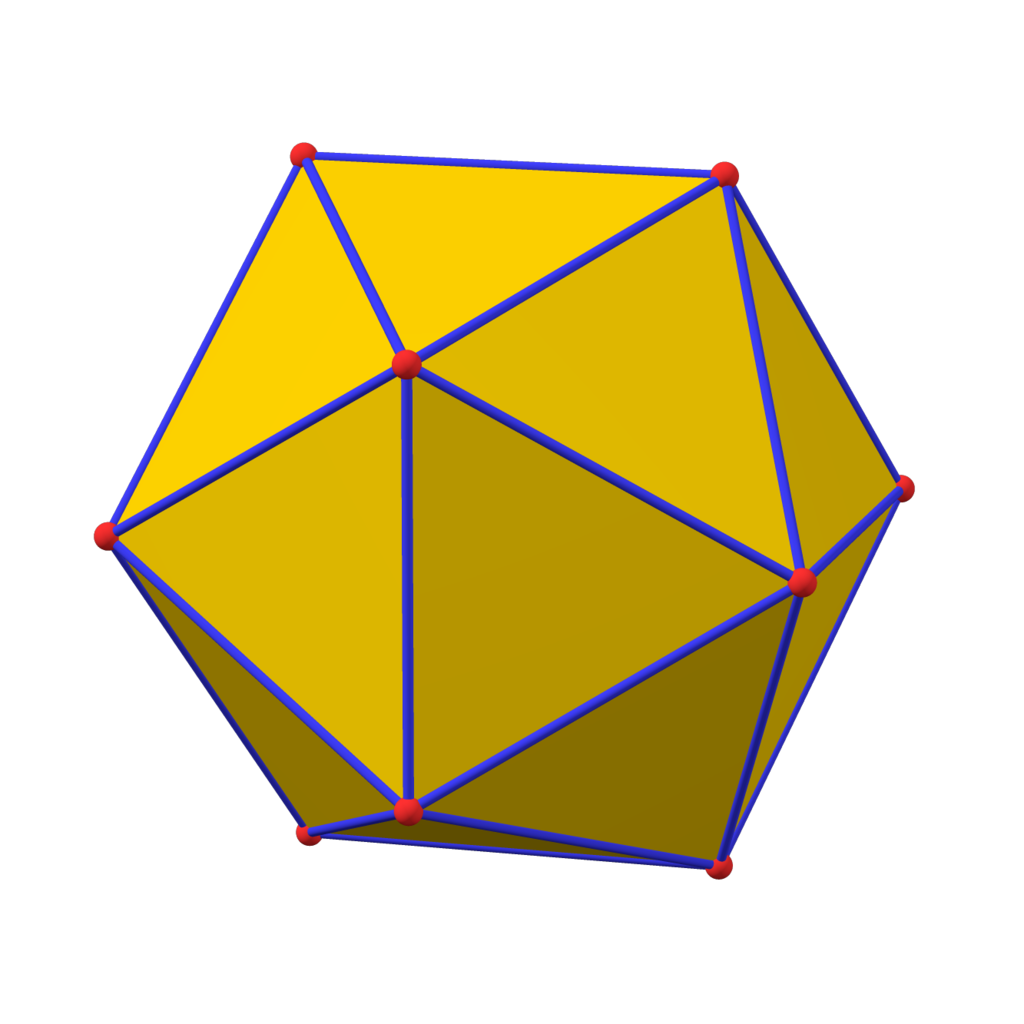
\includegraphics[width=0.25\textwidth]{icosahedron.png}
	\end{center}

	In this shape, there is 20 faces, 12 vertices and 30 edges. We want to know the possible orders of elements in this group, and the number of elements of each order.
\begin{center}
	\begin{tabular}{@{}cc@{}}
		\toprule
		Order & Number of Elements in G   \\ \midrule
		1 	  & 1                         \\
		2	  & 15 \\
		3 	  & 20 \\
		5 	  & 24\\\bottomrule
		\end{tabular}
\end{center}
This gives us a total of $60$ elements. We can verify this with the orbit-stabiliser theorem. For $G$ acting on the vertices, and some vertex $v$, we have $|G| = |\orb(v)| \cdot |\stab(x)| = 12 \cdot 5 = 60$.

To consider the conjugacy classes, we note that two elements are conjugate if they `look the same up to relabelling the icosahedron'.

The elements of order 2 are all conjugate, as are those by order 3. The elements of order 5 split into two conjugacy classes of equal size (12), as the rotations by $\pm \frac{2 \pi}{5}$ are all conjugate and rotations by $\pm \frac{4 \pi}{5}$ are all conjugate, but not to each-other.

We can use this to deduce $G$ is simple. If $H \normal G$, then $|H| = 1 + 15 a + 20b + 12c$ for $a, b \in \{0, 1\}$ and $c \in \{0, 1, 2\}$, but as $|H| \mid 60$ by Lagrange, we get $|H| = 1$ or 60. Thus $G$ is simple.

In fact, $G$ is isomorphic to $A_5$. We will show that the sets $H \leq \{1\}$ for $H \leq G$ a subgroup of order 4 partitions the 15 elements of order 2 into 5 sets of 3. 
\begin{enumerate}
	\item If $|H| = 4$, then $H \cong C_2 \times C_2$ or $H \cong C_4$. But there is no elements of order 4 in $G$, so $H \cong C_2 \times C_2$. Note that this has three elements of order 2.
	\item If $g \in G$ has order 2, then $g \in C_G(g)$ and $|C_G(g)| = \frac{|G||}{|\ccl_G{g}|} = \frac{60}{15} = 4$.
	\item Suppose $e \neq g \in H \cap K$ where $H$ and $K$ are distinct subgroups of order $4$. Then $|C_G(g)| \geq |H \cup K|$ since $H$ and $K$ are abelian, and $|H \cup K| > 4$.
\end{enumerate}
This proves the claim. Now let $G$ act on the set $X$ of subgroups of order 4 by conjugation. We obtain a group homomorphism $\phi:G \rightarrow \sym(X) = S_5$. Then $G$ simple implies either $\kernel \phi = \{e\}$ or $G$. If it was $G$, then we would get that there is a normal subgroup of order $4$m, which is a contradiction. Thus the kernel is trivial, and $G \cong S_5$. Then exactly as before, either $G \cong C_2$ or $G \leq A_5$, and thus $|G| = |A_5| = 60$, so $G \cong A_5$.  
\end{example}

\newchapter{Alternating Groups}

We know from the `Groups' course that two permutations in $S_n$ are conjugate if and only if they have the same cycle type.

\begin{example}[Conjugacy Classes in $S_5$]
	In $S_5$, we have the following:
	\begin{center}
		\begin{tabular}{@{}ccc@{}}
			\toprule
			Cycle Type    & Number of Elements & Sign \\ \midrule
			$1, 1, 1, 1, 1$  & 1   &   $+$  \\ 
			$2, 1, 1, 1$  & 10   &   $-$  \\
			$2, 2, 1$  & 15   &   $+$  \\
			$3, 1, 1$  & 20   &   $+$  \\
			$3, 2$  & 20   &   $-$  \\
			$4, 1$  & 30   &   $-$  \\
			$5$  & 24   &   $+$  \\
			\bottomrule
			\end{tabular}
	\end{center}
	Thus we know the sizes of the conjugacy classes in $S_5$. The same method works in general for $S_n$.
\end{example}

We want to think about the conjugacy classes of $A_n$.

\newsection{Conjugacy Classes \& Simplicity of $A_n$}

One way to think about conjugacy classes is to say that the group acts on itself by conjugation. Then the conjugacy classes correspond to orbits and centralizers correspond to stabilisers.

So it's going to be useful to think about the centralisers of elements in $A_n$. 
Let $g \in A_n$. Then $C_{A_n}(g) = C_{S_n}(g) \cap A_n$. We have then got two cases.
\begin{itemize}
	\item If there exists an odd permutation commuting with $g$, then $|C_{A_n}(g)| = \frac{1}{2}|C_{S_n}(g)|$, and $|\ccl_{A_n}(g)| = |\ccl_{S_n}(g)|$.
	\item  Otherwise, $|C_{A_n}(g)| = |C_{S_n}(g)|$ and $|\ccl_{A_n}(g)| = \frac{1}{2}|\ccl_{S_n}(g)|$.
\end{itemize}

\begin{example}[Conjugacy Classes in $A_5$]
	We can now investigate the conjugacy classes in $A_5$. Note that $(1\ 2)(3\ 4)$ commutes with the odd permutation $(1\ 2)$ and $(1\ 2\ 3)$ commutes with $(4\ 5)$. But if $h \in C_{S_5}(g)$ where $g = (1\ 2\ 3\ 4\ 5)$, then
	$$
(1\ 2\ 3\ 4\ 5) = h (1\ 2\ 3\ 4\ 5) h^{-1} = (h(1)\ h(2)\ h(3)\ h(4)\ h(5)).
	$$
	Thus $h \in \langle g \rangle$, and $|\ccl_{A_5}(g)| = \frac{1}{2}|\ccl_{S_5}(g)| = 12$. Thus $A_5$ has conjugacy classes of size $1, 15, 20, 12, 12$. By the same argument as before, this implies that $A_5$ is simple.
\end{example}

\begin{lemma}[Generators of $A_n$]
	$A_n$ is generated by 3-cycles.
\end{lemma}
\begin{proof}
	We know that each $\sigma \in A_n$ is the product of an even number of transpositions. So it suffices to write the product of any two transpositions as the product of 3-cycles. 

	For $a, b, c, d$ distinct, we have $(a\ b)(b\ c) = (a\ b\ c)$, and $(a\ b)(c\ d) = (a\ c\ b)(a\ c\ d)$.
\end{proof}

\begin{lemma}[3-Cycles are Conjugate in $A_n$]
	If $n \geq 5$, then all $3$-cycles in $A_n$ are conjugate.
\end{lemma}
\begin{proof}
	We claim that every 3-cycle is conjugate to $(1\ 2\ 3)$. Indeed, if $(a\ b\ c)$ is a 3-cycle, then $(a\ b\ c)=\sigma (1\ 2\ 3)\sigma^{-1}$ for some $\sigma \in S_n$. If $\sigma \not \in A_n$, then replace $\sigma$ with $\sigma (4\ 5)$.
\end{proof}

\begin{theorem}[$A_n$ is Simple]
The alternating group $A_n$ is simple for all $n \geq 5$.
\end{theorem}
\begin{proof}
	Let $N \normal A_n$ be a non-trivial subgroup of $A_n$. It suffices to show that $N$ contains a $3$-cycle.
	
	We take some $\sigma \in N$ with $\sigma \neq e$, and write $\sigma$ as the product of disjoint cycles.

	\begin{itemize}
		\item \emph{Case 1}. $\sigma$ contains a cycle of length $r \geq 4$.
	
		Without loss of generality, let $\sigma = (1\ 2\ 3\ \cdots\ r)\tau$. Let $\delta = (1\ 2\ 3)$, then $\delta^{-1} \sigma \delta \in N$, and $\sigma^{-1}\delta^{-1} \sigma \delta \in N$. This can be written $(r\ \cdots\ 2\ 1)(1\ 3\ 2)(1\ 2\ \cdots\ r)(1\ 2\ 3) = (2\ 3\ r)$, which is a three cycle. Then $N$ contains a three cycle.

		\item \emph{Case 2}. $\sigma$ contains two 3-cycles.
		
		Again, without loss of generality say $\sigma = (1\ 2\ 3)(4\ 5\ 6)\tau$. Then let $\delta = (1\ 2\ 4)$, and $\sigma^{-1}\delta^{-1}\sigma \delta = (1\ 3\ 2)(4\ 6\ 5) (1\ 4\ 2)(1\ 2\ 3)(4\ 6\ 5)(1\ 2\ 3) = (1\ 2\ 4\ 3\ 6)$. Then we can apply case 1, and $N$ contains a three cycle.
		\item \emph{Case 3}. $\sigma$ contains two 2-cycles.
		
		Without loss of generality, say $\sigma = (1\ 2)(3\ 4) \tau$. Then let $\delta = (1\ 2\ 3)$. Then $\sigma^{-1}\delta^{-1} \sigma \delta = (1\ 2)(3\ 4)(1\ 3\ 2)(1\ 2)(3\ 4)(1\ 2\ 3) = (1\ 4)(2\ 3)$. Calling this $\pi$, and letting $\epsilon = (2\ 3\ 5)$, then $\pi^{-1} \epsilon^{-1} \pi \epsilon = (1\ 4)(2\ 3)(2\ 5\ 3)(1\ 4)(2\ 3)(2\ 3\ 5) = (2\ 5\ 3)$, so $N$ contains a $3$-cycle. Note that we use $n \geq 5$ here. 
	\end{itemize}
	It remains to consider $\sigma$ where it is a three-cycle. But then $N$ contains a 3-cycle.
\end{proof}

\begin{definition}[Automorphism]
	An \vocab{automorphism} of a group $G$ is an isomorphism $G \rightarrow G$.
\end{definition}

The automorphisms of a group form a subgroup $\aut(G) \leq \sym(G)$.

\newchapter{$p$-Groups and $p$-Subgroups}

Throughout this section, $p$ will denote a fixed prime number.

\begin{definition}[$p$-group]
	A finite group $G$ is a $p$-group if $|G| = p^n$ for $n \in \N$ where $p$ is a prime.
\end{definition}

\newsection{Basic Properties of $p$-Groups}

We will now state some basic properties of $p$-groups that will be used in the following sections.

\begin{theorem}[$p$-groups Have Non-trivial Centers]
	If $G$ is a $p$-group, then $Z(G) \neq \{e\}$.
\end{theorem}
\begin{proof}
	For $g \in G$, we have $|\ccl_G(g)| \cdot |C_G(g)| = |G| = p^n$. So each conjugacy class has size that is a power of $p$. 
	Since $G$ is a union of it's conjugacy classes, 
	\begin{align*}
		|G| &\equiv \#(\text{conj. classes of size 1}) \pmod{p}  \\
\implies 0 &\equiv |Z(G)| \pmod{p}.
	\end{align*}
	In particular, $|Z(g)| > 1$.
\end{proof}

\begin{corollary}[Simple $p$-groups]
	The only simply $p$-group is $C_p$.
\end{corollary}
\begin{proof}
	Let $G$ be a simple $p$-group. Since $Z(G) \normal G$, we have either $Z(G) = \{e\}$ or $G$. The center cannot be trivial by the previous theorem, thus $Z(G) = G$, and the only abelian simple groups are $C_p$.
\end{proof}

\begin{corollary}
	Let $G$ be a $p$-group of order $p^n$. Then $G$ has a subgroup of order $p^r$ for all $0 \leq r \leq n$.
\end{corollary}
\begin{proof}
	We know that any finite group $G$ has a composition series $\{e\} = G_0 \triangleleft G_1 \triangleleft \cdots \triangleleft G_{m - 1} \triangleleft G_m = G$, with each quotient $G_i / G_{i - 1}$ simple. Then $G$ is a $p$-group implies $G_i/G_{i - 1}$ is a $p$-group, and thus $G_i/G_{i - 1} \cong C_p$. Then $|G_i| = p^3$ for all $0 \leq i \leq m$, and $m = n$. 
\end{proof}

\begin{lemma}
	For $G$ a group, if $G/Z(G)$ is cycle, then $G$ is abelian, and $G/Z(G)$ is trivial.
\end{lemma}
\begin{proof}
	Let $gZ(G)$ be a generator for $G/Z(G)$. Then each coset is of the form $g^r Z(G)$ for some $r \in \mathbb{Z}$. Thus $G = \{g^r z \mid r \in \Z, z \in Z(G) \}$.
	Then $(g^{r_1} z_1)(g^{r_2}z_2) = g^{r_1 + r_2} z_1 z_2$ since $z_1$ is in the center.
	We can also write this as $g^{r_1 + r_2}z_2 z_1 =  (g^{r_2} z_2)(g^{r_1} z_1)$, since $z_2$ is also in the center. Thus $G$ is abelian.
\end{proof}

We can now start to consider what various $p$-groups actually look like. We know that a group of order $p$ is cyclic, so we will begin with groups of order $p^2$.

\begin{corollary}[Groups of Order $p^2$]
	If $|G| = p^2$, then $G$ is abelian.
\end{corollary}
\begin{proof}
	The center of $G$ is non-trivial, and by thus by Lagrange, $|Z(G)|$ is either $p$ or $p^2$. If the order was $p^2$, then we would be done. So consider the case $|Z(G)| = p$. Then $|G/Z(G)|$ must have order $p$, but then it is cyclic and contradicts our previous lemma.
\end{proof}

We will leave considering groups of order $p^3$ as an exercise.

\newsection{Sylow Theorems}

Let $G$ be a finite group, and write $|G| = p^a m$ where $p$ is a prime with $p \nmid m$.

\begin{theorem}[First Sylow Theorem]
	The set $\syl_p(G) = \{P \leq G \mid |P| = p^a \}$ of \vocab{Sylow $p$-subgroups} is non-empty.
\end{theorem}
\begin{theorem}[Second Sylow Theorem]
	All elements of $\syl_p(G)$ are conjugate.
\end{theorem}

\begin{theorem}[Third Sylow Theorem]
	The number $n_p = |\syl_p(G)|$ of Sylow $p$-subgroups satisfies $n_p \equiv 1 \pmod{p}$, and $n_p \mid G$. 
\end{theorem}

Proof later on!

\begin{corollary}
	If $n_p = 1$, then the unique Sylow $p$-subgroup is normal.
\end{corollary}
\begin{proof}
Let $g \in G$ and $P \in \syl_p(G)$ Then $gPG^{-1} \leq G$ is another Sylow $p$-subgroup, so we must have $gPg^{-1} = P$, for all $g \in G$. Then $P \normal G$.
\end{proof}

\begin{example}[No Simple Groups of Order 1000]
Let $|G| = 1000 = 2^3 \cdot 5^3$. Then $n_5 \equiv 1 \pmod{5}$, and $n_5 \mid 8$. Checking, we find that $n_5 = 1$, and the unique Sylow $5$-subgroup is normal. Then $G$ is not simple.
\end{example}


\begin{example}[No Simple Groups of Order 132]
	Let $|G| = 132 = 2^3 \cdot 3 \cdot 11$. Then $n_{11} \equiv 1 \pmod{11}$, and $n_{11} \pmod 12$. Then $n_{11} = 1$ or $12$. 

	Suppose $G$ was simple. Then $n_{11} \neq 1$, so $n_{11} = 12$. Now $n_3 \equiv 1 \pmod{3}$, and $n_3 \mid 44$, so $n_3 = 1, 4$ or $22$. But $G$ is simple, and either $n_3 = 4$ or $22$. Supposing $n_3 = 4$, then letting $G$ act on $\syl_3(G)$ by conjugation, we get a group homomorphism $\phi: G \rightarrow S_4$. Then $\kernel(\phi) \normal G$ implies $\kernel(\phi) = \{e\}$ or $G$. It cannot be $G$ by the second Sylow theorem, thus $\phi$ is injective. But then $G \hookrightarrow S_4$, and $132 \leq 24$, which is a contradiction.

	Thus $n_3 = 22$, and $n_11 = 12$. But then counting the $G$ has $22 \cdot (3 - 1) = 44$ elements of order 3, and $12 \cdot (11 - 1) = 120$ elements of order 11. But then $120 + 44 = 164 > 132$, which is a contradiction. Thus there does not exist a simple group of order $132$. 
\end{example}
\end{document}
